\section{}
% For each bridge configuration (quarter, half and full) and each load, make a table 
% showing: weight, voltage reading without weight, voltage reading with weight, 
% Δ𝐸w, Δ𝐸0
% , and the measured strain. Show a sample calculation showing how to 
% calculate the measured strain for each bridge calculation.

\subsection{Quarter Bridge}
% Mass	Voltage reading without weight, Enw	Voltage reading with weight, Ew	delta Ew	delta E0	epsilon
% (kg)	(V)	(V)	V	V	
% 0.05	0.870	0.886	0.016	5.33333E-06	3.09E-06
% 0.1	0.864	0.912	0.048	0.000016	9.28E-06
% 0.2	0.870	0.941	0.071	2.36667E-05	1.37E-05
% 0.5	0.870	1.073	0.203	6.76667E-05	3.92E-05
% 1	0.851	1.270	0.419	0.000139667	8.10E-05
% 1	0.844	1.257	0.413	0.000137667	7.98E-05
% 1	0.864	1.276	0.412	0.000137333	7.96E-05
% 1	0.773	1.192	0.419	0.000139667	8.10E-05
% 1	0.773	1.196	0.423	0.000141	8.18E-05
% 1	0.777	1.202	0.425	0.000141667	8.22E-05

\begin{table}[h]
    \centering
    \caption{Quarter bridge results for various mass loads}
    \label{tab:Q1QuarterBridge}
    \begin{tabular}{cccccc}
        \toprule
        Mass & $E_{nw}$ & $E_w$ & $\Delta E_w$ & $\Delta E_0$ & $\epsilon$ \\
        (kg) & (V) & (V) & (V) & (V) & \\
        \midrule
        0.050 & 0.870 & 0.886 & 0.016 & 5.33E-06 & 3.09E-06 \\
        0.100 & 0.864 & 0.912 & 0.048 & 1.60E-05 & 9.28E-06 \\
        0.200 & 0.870 & 0.941 & 0.071 & 2.37E-05 & 1.37E-05 \\
        0.500 & 0.870 & 1.073 & 0.203 & 6.77E-05 & 3.92E-05 \\
        1.000 & 0.851 & 1.270 & 0.419 & 1.40E-04 & 8.10E-05 \\
        1.000 & 0.844 & 1.257 & 0.413 & 1.38E-04 & 7.98E-05 \\
        1.000 & 0.864 & 1.276 & 0.412 & 1.37E-04 & 7.96E-05 \\
        1.000 & 0.773 & 1.192 & 0.419 & 1.40E-04 & 8.10E-05 \\
        1.000 & 0.773 & 1.196 & 0.423 & 1.41E-04 & 8.18E-05 \\
        1.000 & 0.777 & 1.202 & 0.425 & 1.42E-04 & 8.22E-05 \\
        \bottomrule
    \end{tabular}
\end{table}

Sample calculation for $E_0$ of 0.05 kg load:
\begin{align*}
    E_0 &= \frac{E_{\text{w}} - E_{\text{nw}}}{G} \\
    &= \frac{0.886 - 0.870}{3000} \\ 
    &= \boxed{\qty{5.33E-06}{\volt}}
\end{align*}

Sample calculation for $\epsilon$ of 0.05 kg load:
\begin{equation}
    E_0 = \frac{1}{4} E_{\text{in}} F_{\text{g}}
    (\epsilon_1 - \epsilon_2 - \epsilon_3 + \epsilon_4) \label{eq:epsilon}
\end{equation}

From Fig. \ref{fig:strain gage}, we can see that $\epsilon_2 = \epsilon_3 = \epsilon_4 = 0$ for the quarter bridge configuration. Therefore, the equation simplifies to:
\begin{align*}
    E_0 &= \frac{1}{4} E_{\text{in}} F_{\text{g}}
    (\epsilon_1) \\
    \implies \epsilon &= \frac{4 E_0}{E_{\text{in}} F_{\text{g}}} \\
    \epsilon &= \frac{4 \times 5.33E-06}{3.30 \times 2.09} \\
     &= \boxed{qty{3.09E-06}{}}
\end{align*}


\begin{figure}[h]
    \centering
    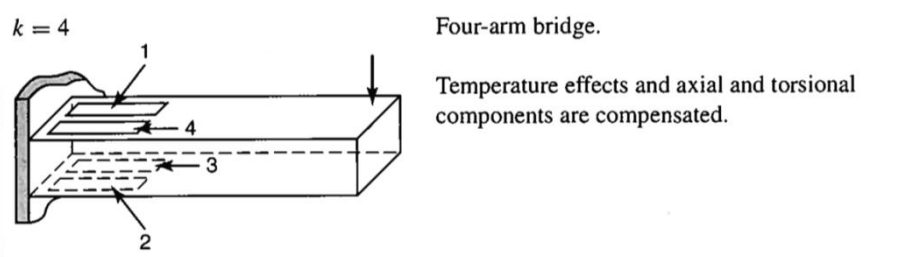
\includegraphics[width=0.5\linewidth]{Sections/Figures/strain gage.png}
    \caption{Strain gage configuration}
    \label{fig:strain gage}
\end{figure}

\subsection{Half Bridge}
% Mass	Voltage reading without weight, Enw	Voltage reading with weight, Ew	delta Ew	delta E0	epsilon
% (kg)	(V)	(V)	V	V	
% 0.050	0.400	0.442	0.042	1.40E-05	4.06E-06
% 0.100	0.396	0.483	0.087	2.90E-05	8.41E-06
% 0.200	0.403	0.567	0.164	5.47E-05	1.59E-05
% 0.500	0.400	0.819	0.419	1.40E-04	4.05E-05
% 1.000	0.396	1.234	0.838	2.79E-04	8.10E-05
% 1.000	0.393	1.234	0.841	2.80E-04	8.13E-05
% 1.000	0.396	1.231	0.835	2.78E-04	8.07E-05
% 1.000	0.390	1.237	0.847	2.82E-04	8.19E-05
% 1.000	0.390	1.234	0.844	2.81E-04	8.16E-05
% 1.000	0.396	1.237	0.841	2.80E-04	8.13E-05
\begin{table}
    \centering
    \caption{Half bridge results for various mass loads}
    \label{tab:Q1HalfBridge}
    \begin{tabular}{cccccc}
        \toprule
        Mass & $E_{nw}$ & $E_w$ & $\Delta E_w$ & $\Delta E_0$ & $\epsilon$ \\
        (kg) & (V) & (V) & (V) & (V) & \\
        \midrule
        0.050 & 0.400 & 0.442 & 0.042 & 1.40E-05 & 4.06E-06 \\
        0.100 & 0.396 & 0.483 & 0.087 & 2.90E-05 & 8.41E-06 \\
        0.200 & 0.403 & 0.567 & 0.164 & 5.47E-05 & 1.59E-05 \\
        0.500 & 0.400 & 0.819 & 0.419 & 1.40E-04 & 4.05E-05 \\
        1.000 & 0.396 & 1.234 & 0.838 & 2.79E-04 & 8.10E-05 \\
        1.000 & 0.393 & 1.234 & 0.841 & 2.80E-04 & 8.13E-05 \\
        1.000 & 0.396 & 1.231 & 0.835 & 2.78E-04 & 8.07E-05 \\
        1.000 & 0.390 & 1.237 & 0.847 & 2.82E-04 & 8.19E-05 \\
        1.000 & 0.390 & 1.234 & 0.844 & 2.81E-04 & 8.16E-05 \\
        1.000 & 0.396 & 1.237 & 0.841 & 2.80E-04 & 8.13E-05 \\
        \bottomrule
    \end{tabular}
\end{table}

Sample calculations for $E_0$ are identical to those for the quarter bridge configuration. 

Sample calculation for $\epsilon$ of 0.05 load is similar to that of the quarter bridge configuration. From Eq. (\ref{eq:epsilon}) and 
Fig. \ref{fig:strain gage}, we can see that $\epsilon_3 = \epsilon_4 = 0$ for the half bridge configuration. Also,
$\epsilon_1 - \epsilon_2 = 2 \epsilon$. Therefore, the equation simplifies to:
\begin{align*}
    E_0 &= \frac{1}{2} E_{\text{in}} F_{\text{g}}
    (\epsilon) \\
    \implies \epsilon &= \frac{2 E_0}{E_{\text{in}} F_{\text{g}}} \\
    \epsilon &= \frac{2 \times 1.40E-05}{3.30 \times 2.09} \\
     &= \boxed{qty{4.06E-06}{}}
\end{align*}

\subsection{Full Bridge}
% Mass	Voltage reading without weight, Enw	Voltage reading with weight, Ew	delta Ew	delta E0	epsilon
% (kg)	(V)	(V)	V	V	
% 0.050	0.274	0.358	0.084	2.80E-05	4.06E-06
% 0.100	0.271	0.435	0.164	5.47E-05	7.93E-06
% 0.200	0.271	0.609	0.338	1.13E-04	1.63E-05
% 0.500	0.271	1.115	0.844	2.81E-04	4.08E-05
% 1.000	0.271	1.969	1.698	5.66E-04	8.21E-05
% 1.000	0.274	1.972	1.698	5.66E-04	8.21E-05
% 1.000	0.274	1.966	1.692	5.64E-04	8.18E-05
% 1.000	0.271	1.966	1.695	5.65E-04	8.19E-05
% 1.000	0.274	1.969	1.695	5.65E-04	8.19E-05
% 1.000	0.277	1.969	1.692	5.64E-04	8.18E-05

\begin{table}[h]
    \centering
    \caption{Full bridge results for various mass loads}
    \label{tab:Q1FullBridge}
    \begin{tabular}{cccccc}
        \toprule
        Mass & $E_{nw}$ & $E_w$ & $\Delta E_w$ & $\Delta E_0$ & $\epsilon$ \\
        (kg) & (V) & (V) & (V) & (V) & \\
        \midrule
        0.050 & 0.274 & 0.358 & 0.084 & 2.80E-05 & 4.06E-06 \\
        0.100 & 0.271 & 0.435 & 0.164 & 5.47E-05 & 7.93E-06 \\
        0.200 & 0.271 & 0.609 & 0.338 & 1.13E-04 & 1.63E-05 \\
        0.500 & 0.271 & 1.115 & 0.844 & 2.81E-04 & 4.08E-05 \\
        1.000 & 0.271 & 1.969 & 1.698 & 5.66E-04 & 8.21E-05 \\
        1.000 & 0.274 & 1.972 & 1.698 & 5.66E-04 & 8.21E-05 \\
        1.000 & 0.274 & 1.966 & 1.692 & 5.64E-04 & 8.18E-05 \\
        1.000 & 0.271 & 1.966 & 1.695 & 5.65E-04 & 8.19E-05 \\
        1.000 & 0.274 & 1.969 & 1.695 & 5.65E-04 & 8.19E-05 \\
        1.000 & 0.277 & 1.969 & 1.692 & 5.64E-04 & 8.18E-05 \\
        \bottomrule
    \end{tabular}
\end{table}

Sample calculations for $E_0$ are identical to those for the quarter bridge configuration.

Sample calculation for $\epsilon$ of 0.05 load is similar to that of the quarter bridge configuration. From Eq. (\ref{eq:epsilon}) and
Fig. \ref{fig:strain gage}, we can see that $\epsilon_1 - \epsilon_2  - \epsilon_3 - \epsilon_4 = 4 \epsilon$. Therefore, the equation simplifies to:
\begin{align*}
    E_0 &= E_{\text{in}} F_{\text{g}}
    (\epsilon) \\
    \implies \epsilon &= \frac{E_0}{E_{\text{in}} F_{\text{g}}} \\
    \epsilon &= \frac{1.40E-05}{3.30 \times 2.09} \\
     &= \boxed{\qty{4.06E-06}{}}
\end{align*}